This part contains results on the enumeration of permutation grid classes. They are useful given that one of the approaches to enumerating permutation classes is through permutation \emph{grid classes}. These are permutation classes themselves but offer additional insight into the structure of the permutations in them. For instance, if a permutation $\sigma$ can be split by a vertical line into a left part and a right part so that the left part (as a subpermutation of $\sigma$) avoids 21 and the right part avoids 12, then $\sigma$ belongs to $\C = \Av(21|12)$, a $1\times 2$ grid class with the left cell being $\Av(21)$ and the right cell being $\Av(12)$. All permutations in $\C$ can be split this way, and all permutations that admit such a gridding belong to $\C$.

The grid class that we just described, in our notation $\Av(21|12)$, was enumerated by Atkinson~\cite{atkinson1998incrdecr}. In~\cite{atkinson1997restricted}, Atkinson used grid classes to enumerate classes such as $\Av(132,4321)$, $\Av(321,2134)$, and $\Av(321,1324)$ (Bevan calls these ``skinny grid classes'' in his thesis~\cite{bevan2015thesis}). In recent years, grid classes were critical to the enumeration of two-by-four classes with two basis elements of length four. See Pantone~\cite{pantone2by4} for enumeration of $\Av(3124,4312)$. Albert, Atkinson, and Brignall used grid classes to enumerate $\Av(2143,4231)$ in~\cite{albert2011enumeration} and three other two-by-four classes in~\cite{albert2012gridclasses}. Albert, Atkinson, and Vatter~\cite{albert2012inflations} use a special kind of grid classes to enumerate three specific permutation classes. Another paper making use of grid classes to enumerate $\Av(4231, 35142, 42513, 351624)$ is by Albert and Brignall~\cite{albert2014schubert}. We also mention Bevan's enumeration of $\Av(4213,2143)$ in~\cite{bevan-new} which utilizes permutation grid classes. 

Generalized grid classes were introduced in Vatter's proof~\cite{vatter11small} of the fact that there are only countably many permutation classes with growth rates below $\kappa \approx 2.20557$ while there are uncountably many permutation classes of growth rate $\kappa$ (note: this is a threshold in the number of permutation classes). On the other hand,  Vatter~\cite{vattercountableuncountable} determines a contant $\xi\approx 2.30522$ such that there are only countably many growth rates of permutation classes below $\xi$ and uncountably many growth rates of permutation classes in any open neighbourhood of $\xi$ (note: this is a threshold in the number of growth rates). The grid classes, whether generalized or not, were instrumental in the characterization of the classes with sub-$\kappa$ growth rates as well as in establishing the threshold $\xi$. The subsequent paper of Pantone and Vatter~\cite{pantonevatter16categorize} characterizes the growth rates below $\xi$ and makes use of grid classes as well.

Apart from enumerating permutation classes, several other applications of grid classes exist, among them~\cite{albert2011enumeration} and~\cite{bevan-new}. We give further examples, with accompanying commentaries, in the next paragraph. For a comprehensive introduction to grid classes and their further uses, see Bevan's PhD thesis~\cite{bevan2015thesis}, Sections 2 and 6 in Part I, as well as parts of the general introduction in Section 1 of Part I.

Because of their more general applicability, the study of grid classes in their own right has emerged in a few directions. For instance, it is conjectured that all monotone grid classes are finitely based, but this is only known for a few special cases, most notably those whose row-column graph is acyclic~\cite{aabrv2013}, and a few other special cases (see~\cite{albert-brignall-2times2, atkinson1997restricted, waton, bevan2015thesis}). In another direction, the role of grid classes with respect to partial well-ordering has been explored in e.g.~\cite{brignall2012pwo, murphy2003pwo, vatter2011pwo}. Finally, while the asymptotic enumeration of monotone grid classes was answered completely by Bevan~\cite{bevan15growth-rates}, exact enumeration is harder, primarily due to the difficulty of handling multiple griddings: that is, enumerating `griddable' objects rather than `gridded' ones. One general result here is that all geometrically griddable classes have rational generating functions~\cite{aabrv2013}, but the move from `gridded' to `griddable' is nonconstructive, instead relying on properties of regular languages.

Since grid classes are often used on the way to enumerating other permutation classes, it would be convenient to be able to enumerate grid classes. Ideally, we would have exact enumerations of classes of the form shown in Figure~\ref{fig:genericgridclass} --- the most generic form of grid classes. For the current level of discussion, Figure~\ref{fig:genericgridclass} also suffices as a definition of a grid class (a grid of permutation classes).

\begin{figure}[ht!]
\begin{center}
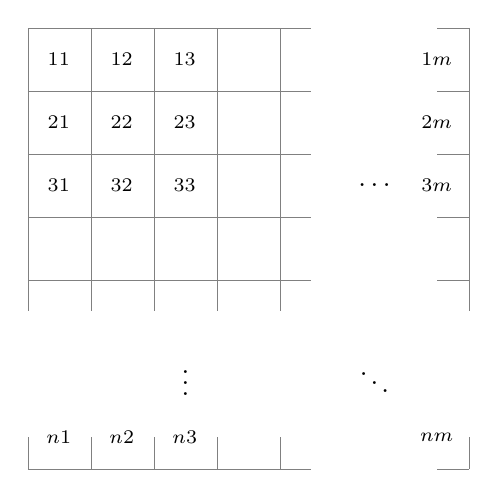
\begin{tikzpicture}[scale=0.8]
  \draw[gray, very thin] (0,0) grid (4,4);
  \draw[gray, very thin] (0,0) -- (0,-0.5);
  \draw[gray, very thin] (1,0) -- (1,-0.5);
  \draw[gray, very thin] (2,0) -- (2,-0.5);
  \draw[gray, very thin] (3,0) -- (3,-0.5);
  \draw[gray, very thin] (4,0) -- (4,-0.5);

  \draw[gray, very thin] (4,4) -- (4.5,4);
  \draw[gray, very thin] (4,3) -- (4.5,3);
  \draw[gray, very thin] (4,2) -- (4.5,2);
  \draw[gray, very thin] (4,1) -- (4.5,1);
  \draw[gray, very thin] (4,0) -- (4.5,0);

  \draw[gray, very thin] (6.5,4) -- (7,4);
  \draw[gray, very thin] (6.5,3) -- (7,3);
  \draw[gray, very thin] (6.5,2) -- (7,2);
  \draw[gray, very thin] (6.5,1) -- (7,1);
  \draw[gray, very thin] (6.5,0) -- (7,0);
  \draw[gray, very thin] (7,4) -- (7,-0.5);

  \draw[gray, very thin] (0,-2.5) -- (0,-3);
  \draw[gray, very thin] (1,-2.5) -- (1,-3);
  \draw[gray, very thin] (2,-2.5) -- (2,-3);
  \draw[gray, very thin] (3,-2.5) -- (3,-3);
  \draw[gray, very thin] (4,-2.5) -- (4,-3);
  \draw[gray, very thin] (0,-3) -- (4.5,-3);

  \draw[gray, very thin] (7,-3) -- (6.5,-3);
  \draw[gray, very thin] (7,-3) -- (7,-2.5);
  \node at (0.5, 3.5){$\C_{11}$};
  \node at (1.5, 3.5){$\C_{12}$};
  \node at (2.5, 3.5){$\C_{13}$};


  \node at (0.5, 2.5){$\C_{21}$};
  \node at (1.5, 2.5){$\C_{22}$};
  \node at (2.5, 2.5){$\C_{23}$};


  \node at (0.5, 1.5){$\C_{31}$};
  \node at (1.5, 1.5){$\C_{32}$};
  \node at (2.5, 1.5){$\C_{33}$};

  \node at (2.5, -1.5){$\vdots$};
  \node at (5.5, -1.5){$\ddots$};
  \node at (5.5, 1.5){$\ldots$};

  \node at (0.5, -2.5){$\C_{n1}$};
  \node at (1.5, -2.5){$\C_{n2}$};
  \node at (2.5, -2.5){$\C_{n3}$};
  \node at (6.5, 3.5){$\C_{1m}$};
  \node at (6.5, 2.5){$\C_{2m}$};
  \node at (6.5, 1.5){$\C_{3m}$};
  \node at (6.5, -2.5){$\C_{nm}$};
\end{tikzpicture}
\end{center}
\caption{A generic format of a generalised grid class, where $\C_{ij}$ are arbitrary but fixed permutation classes.}
\label{fig:genericgridclass}
\end{figure}

The current state of affairs is much more grim. We cannot even enumerate grid classes of the form shown in Figure~\ref{fig:oneC} or in Figure~\ref{fig:allM}. However, there are several important results in this direction. For instance, due to Bevan~\cite{bevan15growth-rates} we at least know the growth rates of monotone grid classes (where every cell is monotone, like Figure~\ref{fig:allM}). The growth rates are equal to the square of the spectral radius of a certain associated row-column graph.

\begin{figure}[ht!]
  \centering
  \begin{subfigure}{0.45\textwidth}
    \centering
    \begin{tikzpicture}[scale=0.6]
  \draw[gray, very thin] (0,0) grid (4,4);
  \draw[gray, very thin] (0,0) -- (0,-0.5);
  \draw[gray, very thin] (1,0) -- (1,-0.5);
  \draw[gray, very thin] (2,0) -- (2,-0.5);
  \draw[gray, very thin] (3,0) -- (3,-0.5);
  \draw[gray, very thin] (4,0) -- (4,-0.5);

  \draw[gray, very thin] (4,4) -- (4.5,4);
  \draw[gray, very thin] (4,3) -- (4.5,3);
  \draw[gray, very thin] (4,2) -- (4.5,2);
  \draw[gray, very thin] (4,1) -- (4.5,1);
  \draw[gray, very thin] (4,0) -- (4.5,0);

  \draw[gray, very thin] (6.5,4) -- (7,4);
  \draw[gray, very thin] (6.5,3) -- (7,3);
  \draw[gray, very thin] (6.5,2) -- (7,2);
  \draw[gray, very thin] (6.5,1) -- (7,1);
  \draw[gray, very thin] (6.5,0) -- (7,0);
  \draw[gray, very thin] (7,4) -- (7,-0.5);

  \draw[gray, very thin] (0,-2.5) -- (0,-3);
  \draw[gray, very thin] (1,-2.5) -- (1,-3);
  \draw[gray, very thin] (2,-2.5) -- (2,-3);
  \draw[gray, very thin] (3,-2.5) -- (3,-3);
  \draw[gray, very thin] (4,-2.5) -- (4,-3);
  \draw[gray, very thin] (0,-3) -- (4.5,-3);

  \draw[gray, very thin] (7,-3) -- (6.5,-3);
  \draw[gray, very thin] (7,-3) -- (7,-2.5);
  \node at (0.5, 3.5){$\M$};
  \node at (1.5, 3.5){$\M$};
  \node at (2.5, 3.5){$\M$};
  \node at (3.5, 3.5){$\M$};


  \node at (0.5, 2.5){$\M$};
  \node at (1.5, 2.5){$\M$};
  \node at (2.5, 2.5){\textcolor{red}{$\C$}};
  \node at (3.5, 2.5){$\M$};


  \node at (0.5, 1.5){$\M$};
  \node at (1.5, 1.5){$\M$};
  \node at (2.5, 1.5){$\M$};
  \node at (3.5, 1.5){$\M$};

  \node at (2.5, -1.5){$\vdots$};
  \node at (5.5, -1.5){$\ddots$};
  \node at (5.5, 1.5){$\ldots$};

  \node at (0.5, -2.5){$\M$};
  \node at (1.5, -2.5){$\M$};
  \node at (2.5, -2.5){$\M$};
  \node at (6.5, 3.5){$\M$};
  \node at (6.5, 2.5){$\M$};
  \node at (6.5, 1.5){$\M$};
  \node at (6.5, -2.5){$\M$};
\end{tikzpicture}
\caption{All cells are monotone except for $\C$, which is a more complex class.}
\label{fig:oneC}
\end{subfigure}\hfill
\begin{subfigure}{0.45\textwidth}
  \centering
  \begin{tikzpicture}[scale=0.6]
  \draw[gray, very thin] (0,0) grid (4,4);
  \draw[gray, very thin] (0,0) -- (0,-0.5);
  \draw[gray, very thin] (1,0) -- (1,-0.5);
  \draw[gray, very thin] (2,0) -- (2,-0.5);
  \draw[gray, very thin] (3,0) -- (3,-0.5);
  \draw[gray, very thin] (4,0) -- (4,-0.5);

  \draw[gray, very thin] (4,4) -- (4.5,4);
  \draw[gray, very thin] (4,3) -- (4.5,3);
  \draw[gray, very thin] (4,2) -- (4.5,2);
  \draw[gray, very thin] (4,1) -- (4.5,1);
  \draw[gray, very thin] (4,0) -- (4.5,0);

  \draw[gray, very thin] (6.5,4) -- (7,4);
  \draw[gray, very thin] (6.5,3) -- (7,3);
  \draw[gray, very thin] (6.5,2) -- (7,2);
  \draw[gray, very thin] (6.5,1) -- (7,1);
  \draw[gray, very thin] (6.5,0) -- (7,0);
  \draw[gray, very thin] (7,4) -- (7,-0.5);

  \draw[gray, very thin] (0,-2.5) -- (0,-3);
  \draw[gray, very thin] (1,-2.5) -- (1,-3);
  \draw[gray, very thin] (2,-2.5) -- (2,-3);
  \draw[gray, very thin] (3,-2.5) -- (3,-3);
  \draw[gray, very thin] (4,-2.5) -- (4,-3);
  \draw[gray, very thin] (0,-3) -- (4.5,-3);

  \draw[gray, very thin] (7,-3) -- (6.5,-3);
  \draw[gray, very thin] (7,-3) -- (7,-2.5);
  \node at (0.5, 3.5){$\M$};
  \node at (1.5, 3.5){$\M$};
  \node at (2.5, 3.5){$\M$};
  \node at (3.5, 3.5){$\M$};


  \node at (0.5, 2.5){$\M$};
  \node at (1.5, 2.5){$\M$};
  \node at (2.5, 2.5){$\M$};
  \node at (3.5, 2.5){$\M$};


  \node at (0.5, 1.5){$\M$};
  \node at (1.5, 1.5){$\M$};
  \node at (2.5, 1.5){$\M$};
  \node at (3.5, 1.5){$\M$};

  \node at (2.5, -1.5){$\vdots$};
  \node at (5.5, -1.5){$\ddots$};
  \node at (5.5, 1.5){$\ldots$};

  \node at (0.5, -2.5){$\M$};
  \node at (1.5, -2.5){$\M$};
  \node at (2.5, -2.5){$\M$};
  \node at (6.5, 3.5){$\M$};
  \node at (6.5, 2.5){$\M$};
  \node at (6.5, 1.5){$\M$};
  \node at (6.5, -2.5){$\M$};
\end{tikzpicture}
\caption{All cells are monotone (increasing or decreasing).}
\label{fig:allM}
\end{subfigure}
\caption{We cannot enumerate either of the two grid classes in~\ref{fig:oneC} and~\ref{fig:allM}.}
\label{fig:wecantdo}
\end{figure}

Approaching the topic from another angle, Albert, Atkinson, Bouvel, Ru\v{s}kuc and Vatter~\cite{aabrv2013} proved that geometrically griddable monotone classes are enumerated by \emph{rational} generating functions. Notice that this result is different from the exact enumeration type of results. And that along two dimensions. First, the authors do exact enumeration in the usual constructive fashion. Second, they assume certain niceness of the grid class --- the monotone classes are geometric and therefore the grid avoids cycles. Still, their result is important and goes to show how unreasonable it is at this point to ask for exact enumeration of arbitrary grid classes.

Lastly, Bevan~\cite{bevan2015thesis} conjectured the generating functions of monotone increasing grid classes of dimension $1\times k$ for some $k$. He also provides a method for enumerating $1\times k$ monotone grid classes in the sense that for any fixed $1\times k$ monotone grid class, he gives a finite procedure that enumerates it.

The aim of Part I of this thesis is to make progress on describing permutation grid classes along the lines of previous research. In Chapter~\ref{chap:catalanjuxt} we pick the simplest possible non-trivial grid classes of the form shown in Figure~\ref{fig:oneC} and enumerate them exactly. They are $1\times 2$ grid classes, also referred to as juxtapositions, of a Catalan class $\C$ with a a monotone class $\M$. In Chapter~\ref{chap:iterjuxt} we choose to prove a result similar in character to that of~\cite{aabrv2013}. We show that all $1\times m$ monotone grid classes with one cell substituted for a context-free class $\C$ admit algebraic generating functions. Our methods allow us to enumerate several new grid classes exactly.

Recall that each permutation in a \emph{grid class} can be drawn into a grid so that the subpermutation in each box is in the class specified by the corresponding cell in a \emph{gridding matrix}. See Figure~\ref{fig:genericgridclass}, where the gridding matrix is represented by a square grid, and Figure~\ref{fig:gridexample}  for an example of permutations from a \emph{monotone grid class} (where each cell in the gridding matrix is a 21-avoider, 12-avoider, or empty).

\newsavebox{\smlmata}
\savebox{\smlmata}{$\left(\begin{smallmatrix} \emptyset & \Av(12)\\ \Av(21) & \emptyset \end{smallmatrix}\right)$}
\newsavebox{\smlmatb}
\savebox{\smlmatb}{$\left(\begin{smallmatrix}\Av(21) & \Av(12) \end{smallmatrix}\right)$}

\begin{figure}[!ht]
\begin{center}
\captionsetup{singlelinecheck=off}
  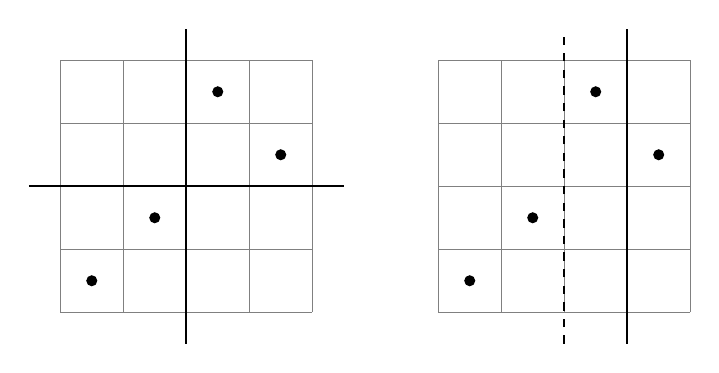
\begin{tikzpicture}[baseline=-0ex,scale=0.8]
  \tikzstyle{vertex}=[circle,fill=black, minimum size=4pt,inner sep=1pt]
  \node[vertex] (v1) at (0.5, 0.5){};
  \node[vertex] (v2) at (1.5,1.5){};
  \node[vertex] (v3) at (2.5, 3.5){};
  \node[vertex] (v4) at (3.5, 2.5){};
  \draw[gray, very thin] (0,0) grid (4,4);
  \draw[thick] (2,-0.5)--(2,4.5);
  \draw[thick] (-0.5,2)--(4.5,2);
  \draw (v1) (v2) (v3) (v4);

  \node[vertex] (v5) at (6.5, 0.5){};
  \node[vertex] (v6) at (7.5, 1.5){};
  \node[vertex] (v7) at (8.5, 3.5){};
  \node[vertex] (v8) at (9.5, 2.5){};
  \draw[gray, very thin] (6,0) grid (10,4);
  \draw[thick, dashed] (8,-0.5)--(8,4.5);
  \draw[thick] (9,-0.5)--(9,4.5);
  \draw (v5) (v6) (v7) (v8);
  \end{tikzpicture}
\caption{\small On the left is the unique gridding of 1243 by the gridding matrix $M =$~\usebox{\smlmata}. On the right are the two griddings of 1243 by $M =$~\usebox{\smlmatb}.}
\label{fig:gridexample}
\end{center}
\end{figure}

Juxtapositions are a simple special case of permutation grid classes. To shift the burden of definitions away from Chapter~\ref{chap:catalanjuxt} and~\ref{chap:iterjuxt}, and as a first step towards enumerating more general grid classes, we now define juxtapositions.

Let $P_i$ and $S_j$ be permutations, for all $1\leq i\leq k$ and $1 \leq j \leq l$. Also, let $\mathcal{U} = \Av(P_1,\ldots,P_k)$ and $\mathcal{V} = \Av(S_1,\ldots,S_\ell)$ be  classes of permutations that avoid $P_1,\ldots, P_k$ and $S_1,\ldots,S_\ell$, respectively. A \emph{juxtaposition class} $\mathcal{W} = \Av(P_1,\ldots,P_k\mid S_1, \ldots, S_\ell)$ of classes $\mathcal{U}$ and $\mathcal{V}$ is the set of permutations whose form is $AB$ with $A\in \mathcal{U}$ and $B \in \mathcal{V}$. We say that $\mathcal{U}$ is on the left-hand side (LHS) of $\mathcal{W}$ and that $\mathcal{V}$ is on the right-hand side (RHS) of $\mathcal{W}$. The diagram on the right in Figure~\ref{fig:gridexample} shows a permutation 1243 from the juxtaposition class $\Av(21|12)$, together with two possible griddings of 1243. An early treatment of juxtapositions can be found in Atkinson's \emph{Restricted permutations}~\cite{atkinson1997restricted}, where the author establishes many fundamental properties. For instance, Atkinson proved that if permutation classes $\C$ and $\C'$ both have finite bases, then their juxtaposition $\C|\C'$ also has a finite basis. We make indirect use of this in Chapter~\ref{chap:catalanjuxt} when we list juxtaposition classes in terms of their bases.
